\documentclass[acmsmall,nonacm]{acmart}
\settopmatter{printacmref=false}
\setcopyright{none}
\renewcommand\footnotetextcopyrightpermission[1]{}

\usepackage{graphicx}
\graphicspath{{../figures/}}
\usepackage{booktabs}
\usepackage{mdframed}

% Coloured callout boxes
\newmdenv[backgroundcolor=blue!8, linecolor=blue!40, linewidth=1pt,
          roundcorner=4pt, skipabove=6pt, skipbelow=6pt]{infobox}
\newmdenv[backgroundcolor=orange!10, linecolor=orange!50, linewidth=1pt,
          roundcorner=4pt, skipabove=6pt, skipbelow=6pt]{analogybox}
\newmdenv[backgroundcolor=green!8, linecolor=green!40, linewidth=1pt,
          roundcorner=4pt, skipabove=6pt, skipbelow=6pt]{keypoint}

% ─── METADATA ────────────────────────────────────────────────────────────────
\title{Plain-English Companion to\\``Fourier Neural Operators for 2D Navier--Stokes''}

\author{Ian Havill, Hugh Baldwin, and Aaron Chen}
\affiliation{\institution{Occidental College}\city{Los Angeles}\state{CA}\country{USA}}

\date{May 2026}

% ─── DOCUMENT ────────────────────────────────────────────────────────────────
\begin{document}

\begin{abstract}
A plain-English companion to our technical report on Fourier Neural Operators
for 2D Navier--Stokes prediction.
Every concept is explained from scratch with analogies before any mathematics
appears.
Includes a full glossary of technical terms.
\end{abstract}

\maketitle

\begin{infobox}
\textbf{What this document is.}
The formal report uses technical language for the professor.
This companion explains everything in plain English so \emph{we}
can follow along.
Read them side by side, or read this first.
\end{infobox}

% ─── ABSTRACT IN PLAIN ENGLISH ───────────────────────────────────────────────
\section*{What We Did --- In One Paragraph}

We trained two AI models to watch a swirling fluid (think smoke rings or water
spinning in a sink) and predict what it will look like one moment later.
The first model, called FNO, was designed specifically with fluid physics in mind.
The second, called U-Net, is a general-purpose image model we used as a
comparison point.

FNO won on every single metric: it was three times more accurate, ran more than
twice as fast, and used six times fewer ``brain cells'' (parameters).
On top of that, FNO could handle pictures of the fluid at resolutions it had
\emph{never seen during training} and still did a great job --- U-Net fell apart
completely at those new resolutions.

The big takeaway: when you design an AI model that understands the \emph{shape}
of the problem it is solving (fluid physics), it beats a generic model even if
that generic model is much larger.

% ─── SECTION 1 ───────────────────────────────────────────────────────────────
\section{Introduction --- Why Does Any of This Matter?}

\subsection{Simulating Fluids Is Expensive}

Fluids (liquids and gases) follow rules that scientists have known for over 150
years --- the Navier--Stokes equations.
These equations are correct and precise, but actually \emph{solving} them
on a computer is brutally slow.

\begin{analogybox}
\textbf{Analogy.}
Imagine a weather forecast that requires a supercomputer running for six hours
just to tell you what tomorrow looks like.
That is roughly the situation with high-fidelity fluid simulation.
The equations are not wrong; they are just expensive.
\end{analogybox}

To predict the weather for the next 24 hours at high resolution, scientists
divide the atmosphere into millions of tiny boxes, apply the equations to each
box, and step forward in time --- millions of times.
This works, but it takes enormous computing resources.

\subsection{What We Want Instead}

Instead of solving the equations from scratch every time, we want to
\emph{train} a neural network to look at a snapshot of the fluid and
immediately predict the next snapshot --- skipping all the expensive arithmetic.

This is called a \textbf{surrogate model}: it \emph{stands in} for the real
simulation.
If it works, a single forward pass through the neural network (milliseconds)
replaces the expensive numerical solver (minutes to hours).

\subsection{The Catch}

The tricky part is that the fluid is represented as a \emph{grid of values}
(a 2D image, basically).
If you train a standard image neural network at one image resolution, it
generally cannot handle a different resolution without retraining.
That is a big problem if you want to use the same model at different scales.

FNO was designed to solve this problem by working in \emph{frequency space}
instead of pixel space.
We will explain exactly what that means in Section~\ref{sec:background}.

% ─── SECTION 2 ───────────────────────────────────────────────────────────────
\section{Background --- Building Blocks}
\label{sec:background}

\subsection{What Is a Vorticity Field?}

We do not directly track how fast every tiny piece of fluid is moving.
Instead, we track \textbf{vorticity} --- a number at every point in the fluid
that describes how much the fluid is \emph{spinning} there.

\begin{analogybox}
\textbf{Analogy.}
Picture a river.
Where the water flows straight, vorticity is near zero.
Where it curls into a whirlpool, vorticity is large.
Positive vorticity = spinning clockwise;
negative vorticity = spinning counter-clockwise.
\end{analogybox}

In our case, the fluid lives on a square grid ($128 \times 128$ points).
Each grid point holds one vorticity number.
So one ``snapshot'' of the fluid is just a $128 \times 128$ grid of numbers ---
essentially a grayscale image where brightness = vorticity.

\subsection{What Are the Navier--Stokes Equations?}

The Navier--Stokes equations describe how fluid velocity changes over time.
In plain terms, the equation says:

\begin{center}
\emph{``How the fluid's motion changes right now''} \\[2pt]
$=$ \emph{``How it is pushing itself around''} \\[2pt]
$+$ \emph{``How pressure is pushing it''} \\[2pt]
$+$ \emph{``How viscosity (thickness) slows it down''} \\[2pt]
$+$ \emph{``Any external force acting on it''}
\end{center}

The formal version looks like this:
\[
  \frac{\partial \mathbf{u}}{\partial t} + (\mathbf{u} \cdot \nabla)\mathbf{u}
  = -\nabla p + \nu \nabla^2 \mathbf{u} + \mathbf{f}
\]
Each symbol maps directly onto the plain-English list above.
$\mathbf{u}$ is velocity, $p$ is pressure, $\nu$ is viscosity (how thick the
fluid is --- honey has high $\nu$, air has low $\nu$), and $\mathbf{f}$ is
external force.

The reason this is hard is the middle term on the left, $(\mathbf{u} \cdot
\nabla)\mathbf{u}$: the fluid's own motion affects its future motion (it is
\emph{nonlinear}).
That self-interaction is what causes chaotic, turbulent behaviour.

\subsection{Kolmogorov Forcing --- Why the Fluid Swirls}

Our dataset uses a specific external force called \textbf{Kolmogorov forcing}:
a sinusoidal push that continuously pumps energy into the fluid at a
large spatial scale (imagine someone slowly waving a giant paddle back and
forth).
At the viscosity we use ($\nu = 10^{-4}$, i.e., very thin fluid), that energy
cascades down to smaller and smaller scales, creating complex swirling patterns
--- 2D turbulence.

The fluid in our dataset is not a real physical substance like water or air; it
is a dimensionless benchmark designed to have the right level of complexity for
testing neural networks.

\subsection{What Is a Neural Operator?}

A standard neural network takes in a fixed-length list of numbers and outputs
another fixed-length list.
If you train it on $128 \times 128$ images, you cannot feed it a $256 \times
256$ image.

A \textbf{neural operator} is different: it is designed to map one
\emph{function} to another function, regardless of how finely that function is
sampled.

\begin{analogybox}
\textbf{Analogy.}
A regular neural network is like a calculator that only works on numbers between
0 and 100.
A neural operator is like a formula: it works for any input, no matter how you
choose to measure it.
\end{analogybox}

For fluids, this means: train on $128 \times 128$, then apply to $256 \times
256$ --- no retraining needed.
FNO is one way to build a neural operator.

\subsection{How FNO Works --- Step by Step}

FNO's key insight is that fluid dynamics is \emph{smooth at large scales}:
the big swirling patterns (low frequencies) carry most of the physically
important information.
FNO exploits this by doing its main computation in frequency space.

\paragraph{Step 1 --- FFT.}
Take the $128 \times 128$ vorticity grid and apply a 2D Fast Fourier Transform
(FFT).
This converts the image from ``how much vorticity at each grid point''
into ``how much of each swirling pattern is present.''
Low frequencies = large, smooth swirls; high frequencies = fine, rapid wiggles.

\paragraph{Step 2 --- Truncate.}
Throw away everything above frequency mode 12 in each direction.
We keep only the 12 lowest-frequency components --- the large-scale structure.
This dramatically reduces the amount of information to process and acts as a
physics-motivated compression.

\paragraph{Step 3 --- Multiply by learned weights.}
Each kept frequency mode is multiplied by a learned complex number.
These complex weights are what the training process optimises.
Conceptually, this is the model learning ``how much to amplify or dampen each
frequency when stepping forward in time.''

\paragraph{Step 4 --- Inverse FFT.}
Convert back from frequency space to grid space.
The result is a transformed vorticity field at the original resolution.

\paragraph{Step 5 --- Add a local correction.}
A standard $1 \times 1$ convolution is added in parallel to the Fourier step.
This handles anything that is very local (fine-grained effects that the
truncated frequencies missed).

\paragraph{Why this is resolution-independent.}
The FFT produces frequency components; their physical meaning does not change
when you use a finer or coarser grid.
So the learned weights remain valid at any resolution.
That is the core reason FNO can do zero-shot super-resolution.

\subsection{How U-Net Works}

U-Net is a classic convolutional encoder--decoder.
Think of it as a ``zoom out, transform, zoom back in'' pipeline:

\begin{enumerate}
  \item \textbf{Encoder}: repeatedly shrink the image by half while doubling
        the number of feature channels. Four times = down to $8 \times 8$ with
        512 channels.
  \item \textbf{Bottleneck}: the most compressed representation of the input.
  \item \textbf{Decoder}: upsample back to the original size, step by step.
        At each step, paste in the matching encoder features (skip connections)
        to recover fine detail.
\end{enumerate}

U-Net is extremely good at image-to-image tasks and is the de facto standard in
medical image segmentation.
The limitation: all operations use fixed-size $3 \times 3$ kernels that look at
a specific physical neighbourhood.
When the resolution changes, those kernels cover a different physical area,
which is why U-Net does not generalise across resolutions.

% ─── SECTION 3 ───────────────────────────────────────────────────────────────
\section{Dataset --- What We Actually Fed the Models}

\subsection{Where the Data Comes From}

We used a publicly available dataset from the neuraloperator project, downloaded
from Zenodo (a data-sharing platform for scientists).
File: \texttt{nsforcing\_128.tgz}, about 1.5 GB.

\subsection{What One Training Example Looks Like}

Each example is a pair of two $128 \times 128$ grids:
\begin{itemize}
  \item \textbf{Input} $x$: the vorticity field right now.
  \item \textbf{Target} $y$: the vorticity field one timestep later.
\end{itemize}
The model's job: look at $x$, predict $y$.

\subsection{What the Data Looks Like}

The input fields are calm: numbers mostly between $-0.76$ and $0.82$.
The target fields are more energetic: numbers between $-3.49$ and $3.93$.
This makes sense physically --- the Kolmogorov forcing is continuously pumping
energy in, so the fluid is getting more turbulent over time.

\begin{keypoint}
\textbf{Key point.}
The targets are roughly $20\times$ more variable than the inputs.
This means the model cannot just copy the input and call it done ---
it needs to actually predict the physics.
\end{keypoint}

We have 10{,}000 training pairs and 2{,}000 test pairs.

\begin{figure}[t]
  \centering
  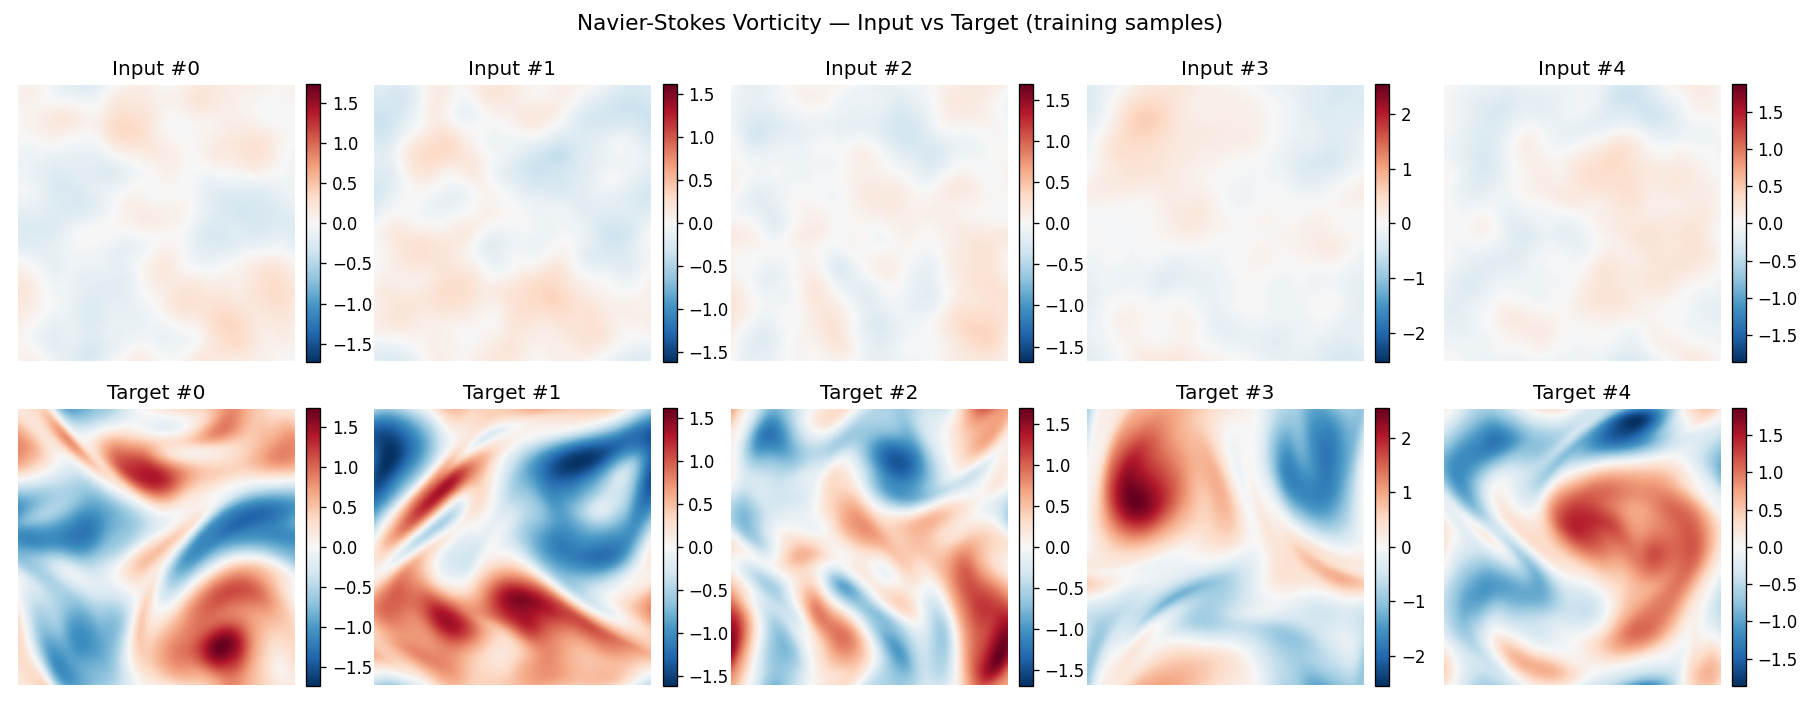
\includegraphics[width=\linewidth]{sample_pairs.png}
  \caption{\textbf{What the data looks like.}
           Five examples from the training set.
           \textbf{Top row:} the input vorticity field the model sees.
           \textbf{Bottom row:} the target field it must predict, one timestep
           later.
           Red = fluid spinning clockwise; blue = fluid spinning
           counter-clockwise; white = not spinning.
           Notice the bottom row is much more dramatic --- more red and blue,
           bigger patches --- because the fluid has become more turbulent.}
  \label{fig:sample_pairs}
\end{figure}

% ─── SECTION 4 ───────────────────────────────────────────────────────────────
\section{Methods --- How We Trained Everything}

\subsection{The Loss Function}

During training, after the model makes a prediction $\hat{u}$, we need to
measure how wrong it was compared to the true answer $u$.
We use \textbf{relative $L^2$ error}:
\[
  \text{error} = \frac{\|\hat{u} - u\|_2}{\|u\|_2}
\]
In plain English: compute the size of the mistake, then divide by the size of
the true answer.
This gives a percentage-like score:
\begin{itemize}
  \item $1.0$ = your prediction is as wrong as a random guess (terrible).
  \item $0.1$ = your mistake is 10\% the size of the true answer (decent).
  \item $0.03$ = your mistake is only 3\% the size (great).
\end{itemize}

\subsection{Training Details}

Both models were trained for 100 epochs (100 full passes over the training set).
We used the Adam optimiser --- a standard recipe for updating the model's
weights to reduce error --- starting with a learning rate of $10^{-3}$ that
slowly decays to $10^{-5}$ over training (cosine schedule).

\begin{analogybox}
\textbf{Analogy --- learning rate.}
The learning rate controls how big a step you take when adjusting the model
after each mistake.
Too large: you overshoot and never settle.
Too small: you take forever.
Cosine scheduling starts large (fast learning) and gradually slows down
(fine-tuning), like how you take big strides to cross a room and then small
careful steps when threading a needle.
\end{analogybox}

Hardware: an NVIDIA RTX 2060 GPU (6 GB video memory), which is a mid-range
gaming card --- not a supercomputer.
Both models trained overnight.

\subsection{What ``Parameters'' Are}

A neural network is basically a huge collection of numbers (called
\textbf{parameters} or \textbf{weights}).
Training adjusts these numbers until the network makes good predictions.
More parameters = more capacity to learn complex patterns, but also more memory
and slower inference.

\begin{itemize}
  \item FNO: \textbf{4.7 million} parameters
  \item U-Net: \textbf{31 million} parameters (6.6$\times$ more)
\end{itemize}

% ─── SECTION 5 ───────────────────────────────────────────────────────────────
\section{Results --- What We Found}

\subsection{Main Results: Accuracy and Speed}

Table~\ref{tab:standard} summarises the head-to-head comparison.

\begin{table}[t]
  \centering
  \caption{Head-to-head comparison on the test set.
           Lower rel-$L^2$ = more accurate.
           Higher throughput = faster.}
  \label{tab:standard}
  \begin{tabular}{lcc}
    \toprule
    & \textbf{FNO} & \textbf{U-Net} \\
    \midrule
    Parameters          & 4.7M           & 31M \\
    Rel-$L^2$ error     & \textbf{0.035} & 0.103 \\
    Throughput (samp/s) & \textbf{499}   & 227 \\
    Latency (ms/samp)   & \textbf{2.0}   & 4.4 \\
    \bottomrule
  \end{tabular}
\end{table}

In plain English:
\begin{itemize}
  \item \textbf{FNO's error is 3.5\%} of the target's magnitude.
        U-Net's is 10.3\%. FNO is about $3\times$ more accurate.
  \item FNO processes \textbf{499 test samples per second};
        U-Net manages 227. FNO is $2.2\times$ faster.
  \item Each FNO prediction takes \textbf{2 milliseconds}.
        U-Net takes 4.4 ms.
  \item FNO achieves all of this with \textbf{6.6$\times$ fewer parameters}.
\end{itemize}

\begin{keypoint}
\textbf{Why does FNO win on speed \emph{and} accuracy?}
FNO's Fourier layers are implemented using the FFT algorithm, which is extremely
efficient.
U-Net's convolutions operate at full $128\times128$ resolution at every level.
FNO's computation is concentrated on the 12 most important frequencies ---
most of the work happens in a much smaller space.
\end{keypoint}

\subsection{Looking at the Predictions}

Figure~\ref{fig:predictions} shows six test examples from worst to best FNO
performance (the number below each column is the relative $L^2$ score for that
sample).

\begin{figure}[t]
  \centering
  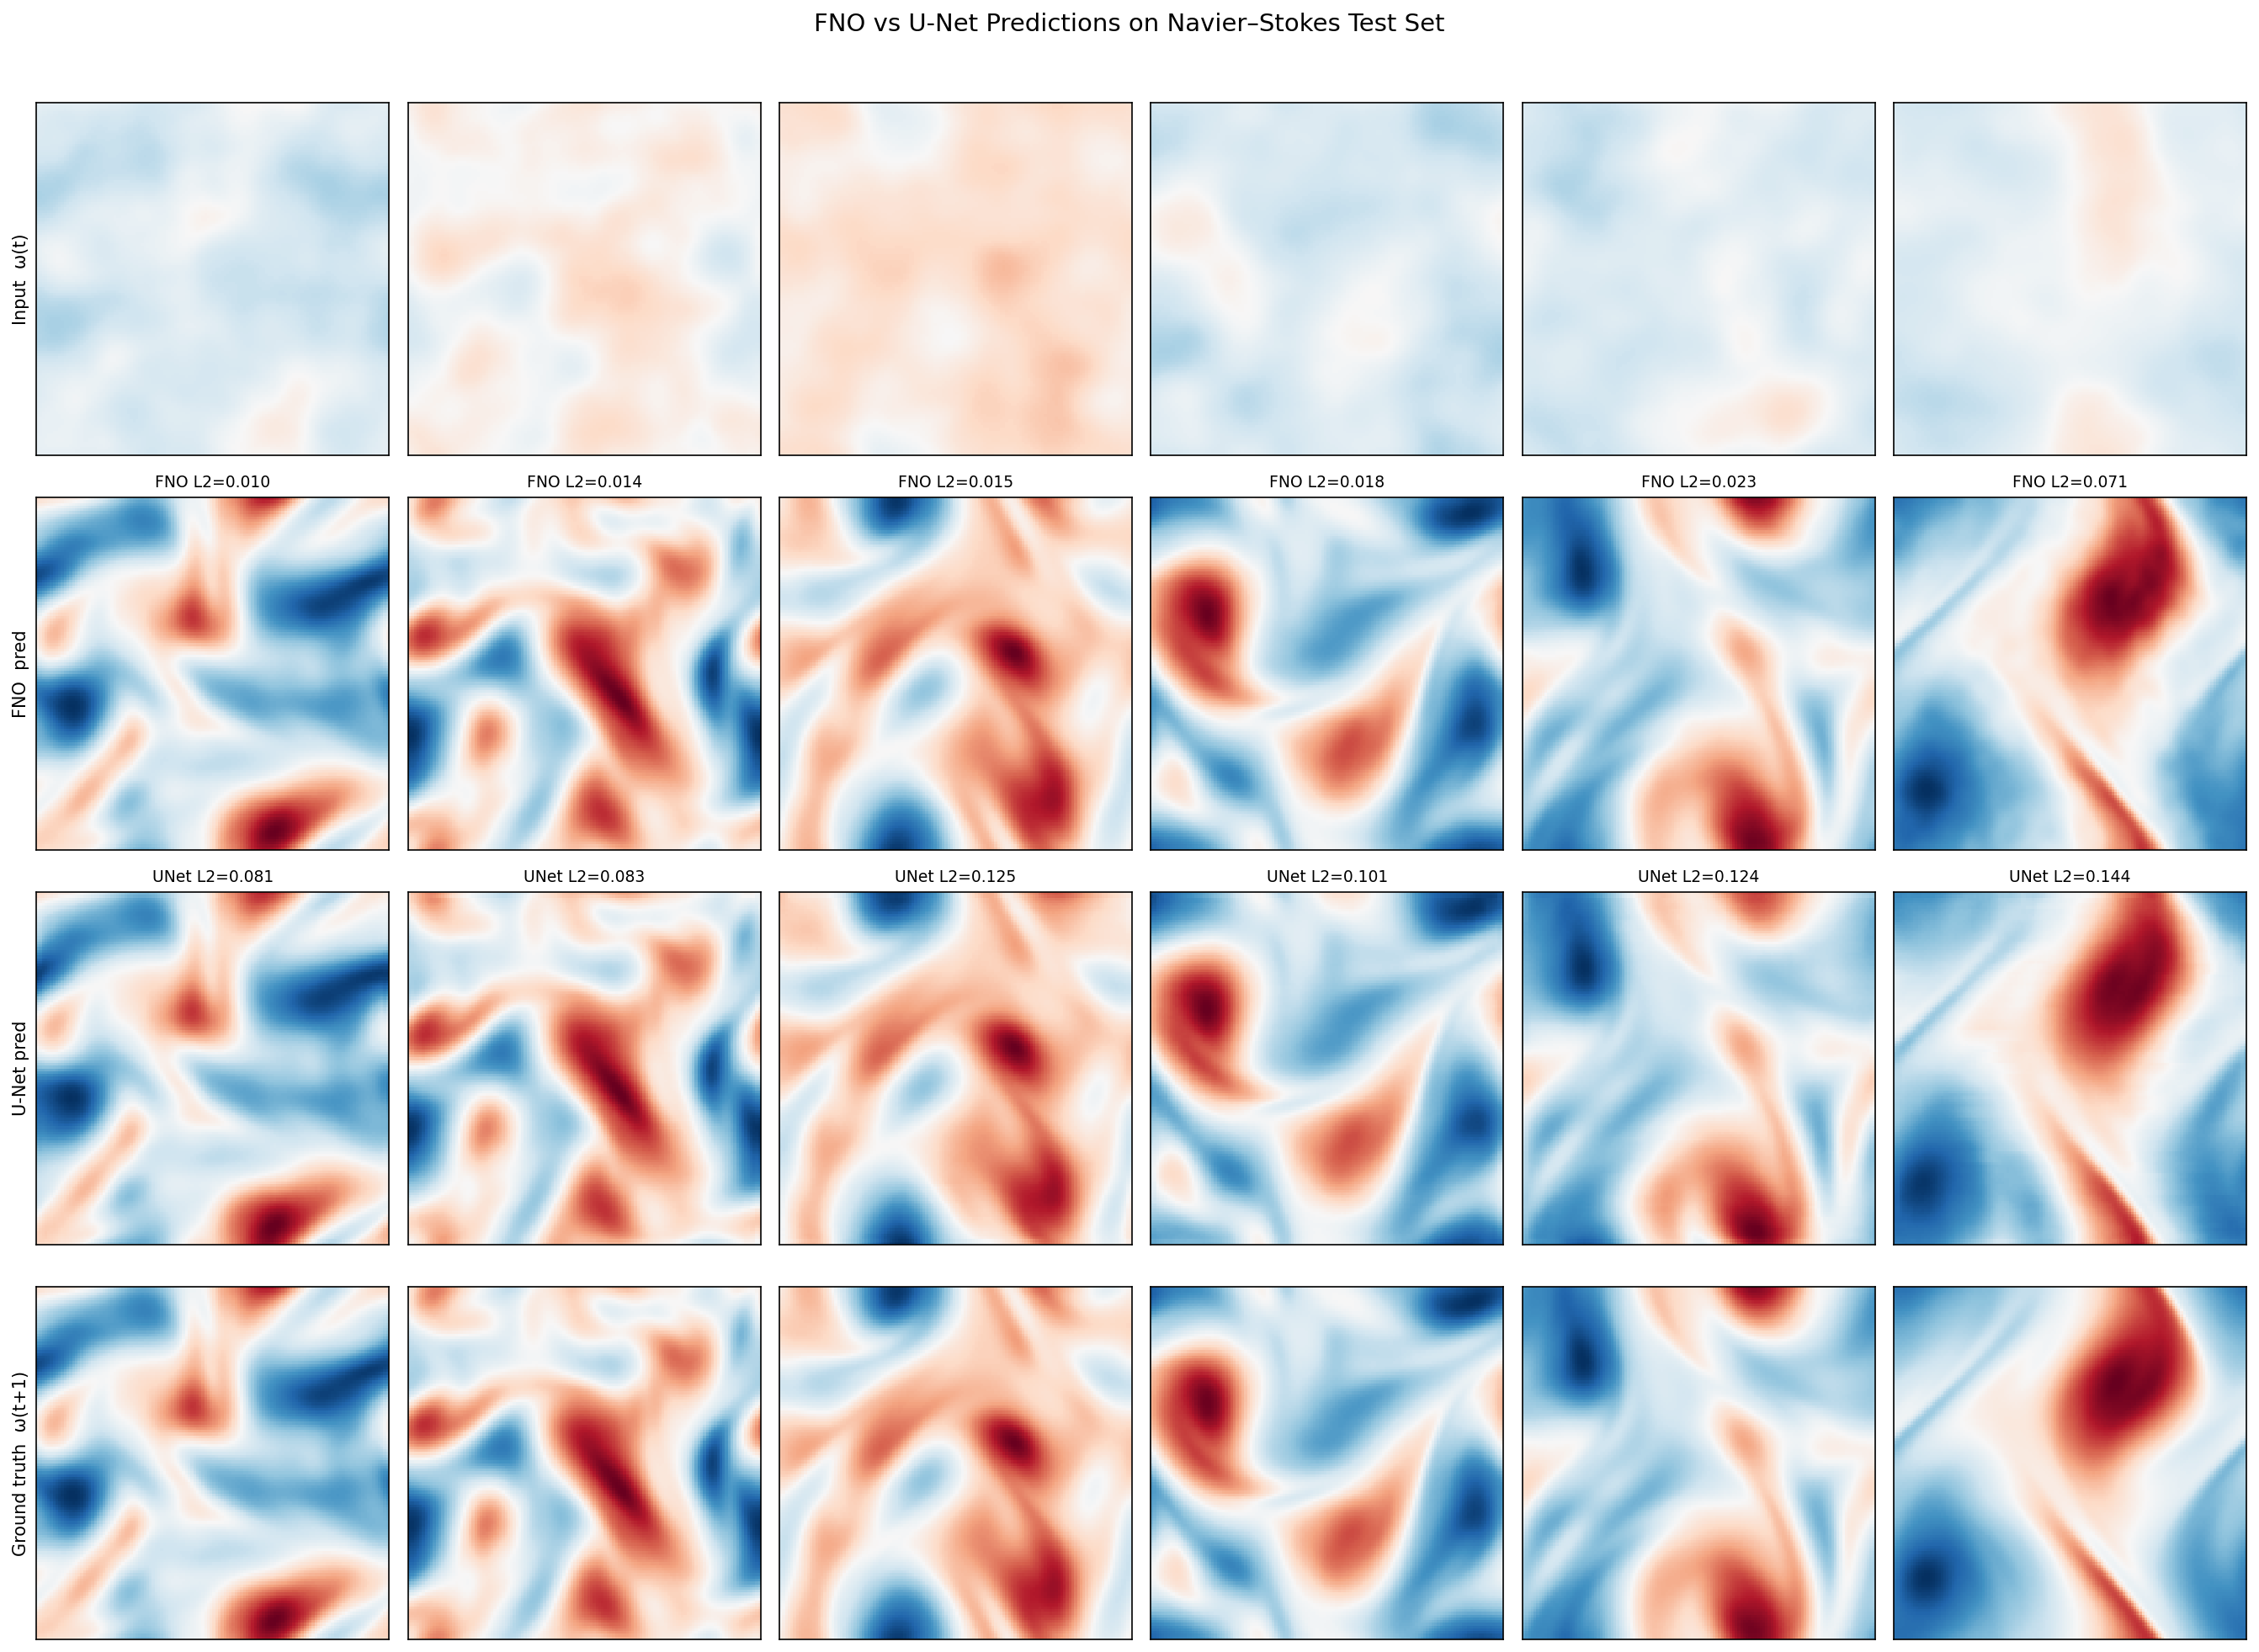
\includegraphics[width=\linewidth]{predictions.png}
  \caption{\textbf{Side-by-side predictions on six test samples.}
           \textbf{Row 1 (Input):} what the model is given.
           \textbf{Row 2 (FNO):} FNO's prediction of the next timestep.
           \textbf{Row 3 (U-Net):} U-Net's prediction.
           \textbf{Row 4 (Truth):} what actually happens next.
           FNO's predictions look almost identical to the ground truth.
           U-Net captures the rough shape but blurs out fine details.}
  \label{fig:predictions}
\end{figure}

\subsection{Where the Errors Are}

Figure~\ref{fig:error_maps} shows \emph{where} each model makes mistakes.
Bright = big error; dark = small error.

\begin{figure}[t]
  \centering
  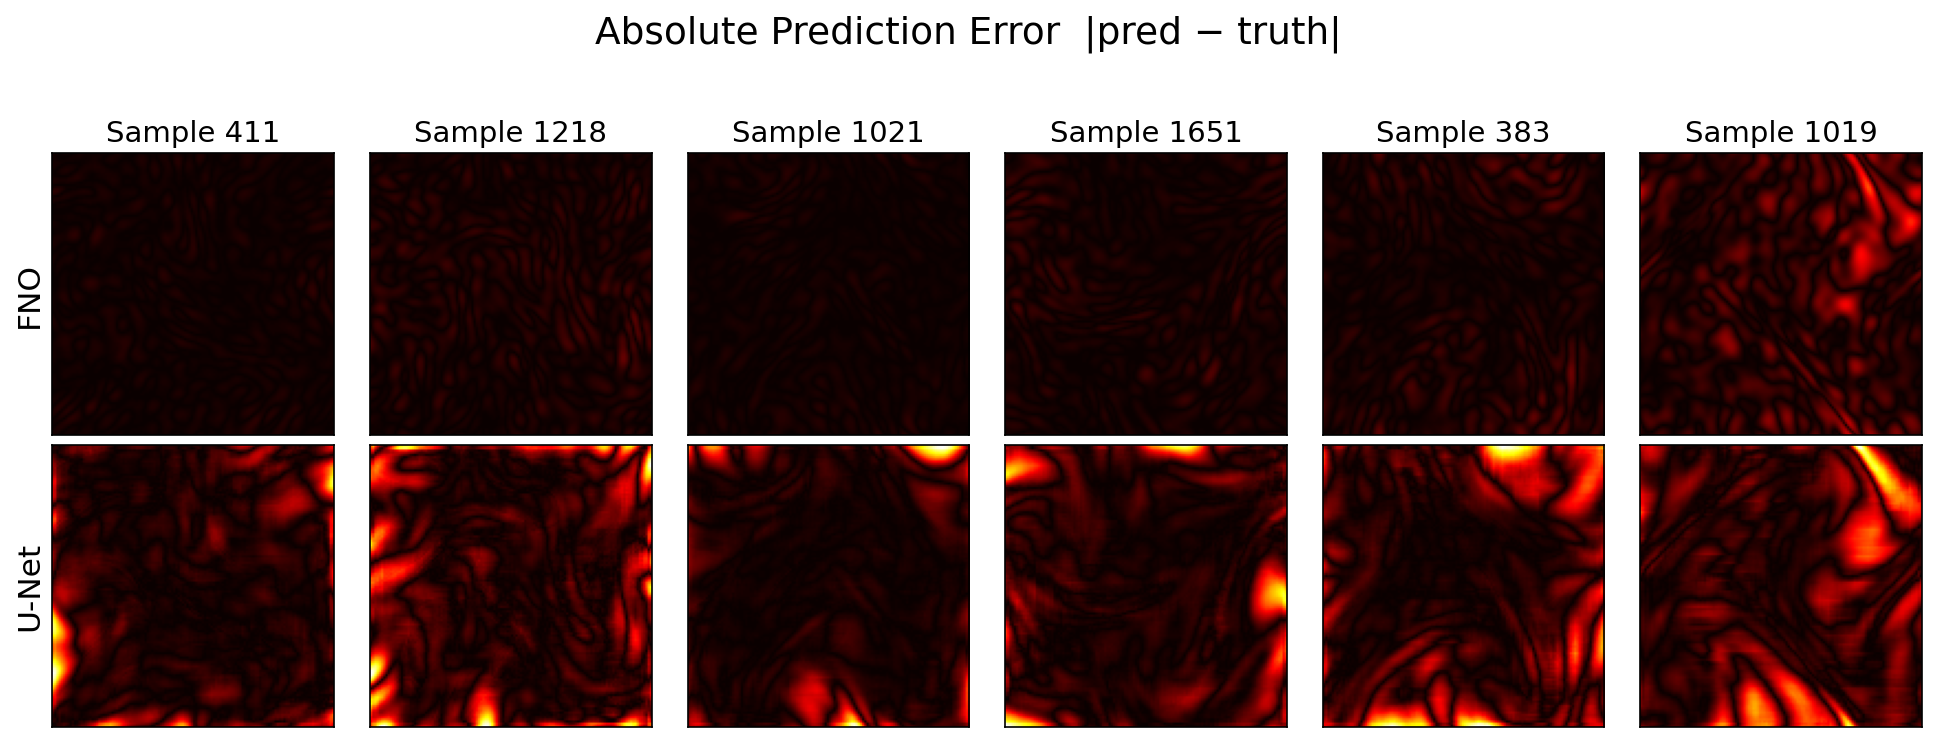
\includegraphics[width=\linewidth]{error_maps.png}
  \caption{\textbf{Error maps: where each model goes wrong.}
           \textbf{Top row (FNO):} errors are small and spread evenly.
           \textbf{Bottom row (U-Net):} errors are large and concentrated
           at the edges of vortices --- exactly the hardest parts, where
           the physics changes most rapidly.}
  \label{fig:error_maps}
\end{figure}

\subsection{How Consistent Are the Models?}

Figure~\ref{fig:error_hist} shows the distribution of errors across all 2{,}000
test samples --- like a grade distribution for each model.

\begin{figure}[t]
  \centering
  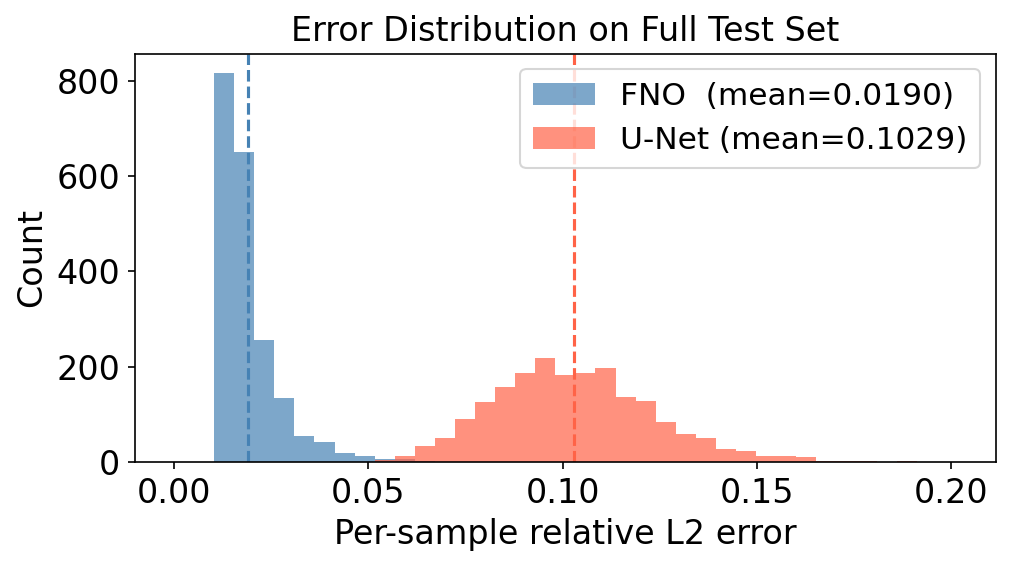
\includegraphics[width=\linewidth]{error_histogram.png}
  \caption{\textbf{Error distribution across the full test set.}
           \textbf{Blue (FNO):} most samples clustered tightly near 0.035.
           \textbf{Red (U-Net):} spread much wider.
           Not only is U-Net less accurate on average, it is also less
           \emph{reliable}.}
  \label{fig:error_hist}
\end{figure}

\subsection{Zero-Shot Super-Resolution --- The Coolest Result}

\begin{infobox}
\textbf{What ``zero-shot super-resolution'' means.}
Both models were trained \emph{only} on $128 \times 128$ images.
We then asked them to make predictions at completely different resolutions ---
$64 \times 64$ (half the size) and $256 \times 256$ (double the size) ---
\textbf{without any additional training}.
This is called ``zero-shot'' because the model gets zero examples at the new
resolution.
\end{infobox}

Table~\ref{tab:superres} shows the results.

\begin{table}[t]
  \centering
  \caption{Zero-shot super-resolution: errors at unseen resolutions.
           The model only trained on the $128\times128$ row.}
  \label{tab:superres}
  \begin{tabular}{lcc}
    \toprule
    Resolution          & FNO error & U-Net error \\
    \midrule
    $64\times64$        & \textbf{0.019} & 0.476 \\
    $128\times128$ (trained on) & \textbf{0.019} & 0.103 \\
    $256\times256$      & \textbf{0.019} & 0.594 \\
    \bottomrule
  \end{tabular}
\end{table}

FNO's error is \textbf{literally identical} across all three resolutions.
It does not care how many pixels you give it --- it is solving the same
underlying physics problem.

U-Net's error at $256 \times 256$ is $0.594$ --- worse than a coin flip
(recall, $1.0$ = random guess).
Its $64 \times 64$ error is $0.476$.
At both unseen resolutions, U-Net essentially fails.

\begin{figure}[t]
  \centering
  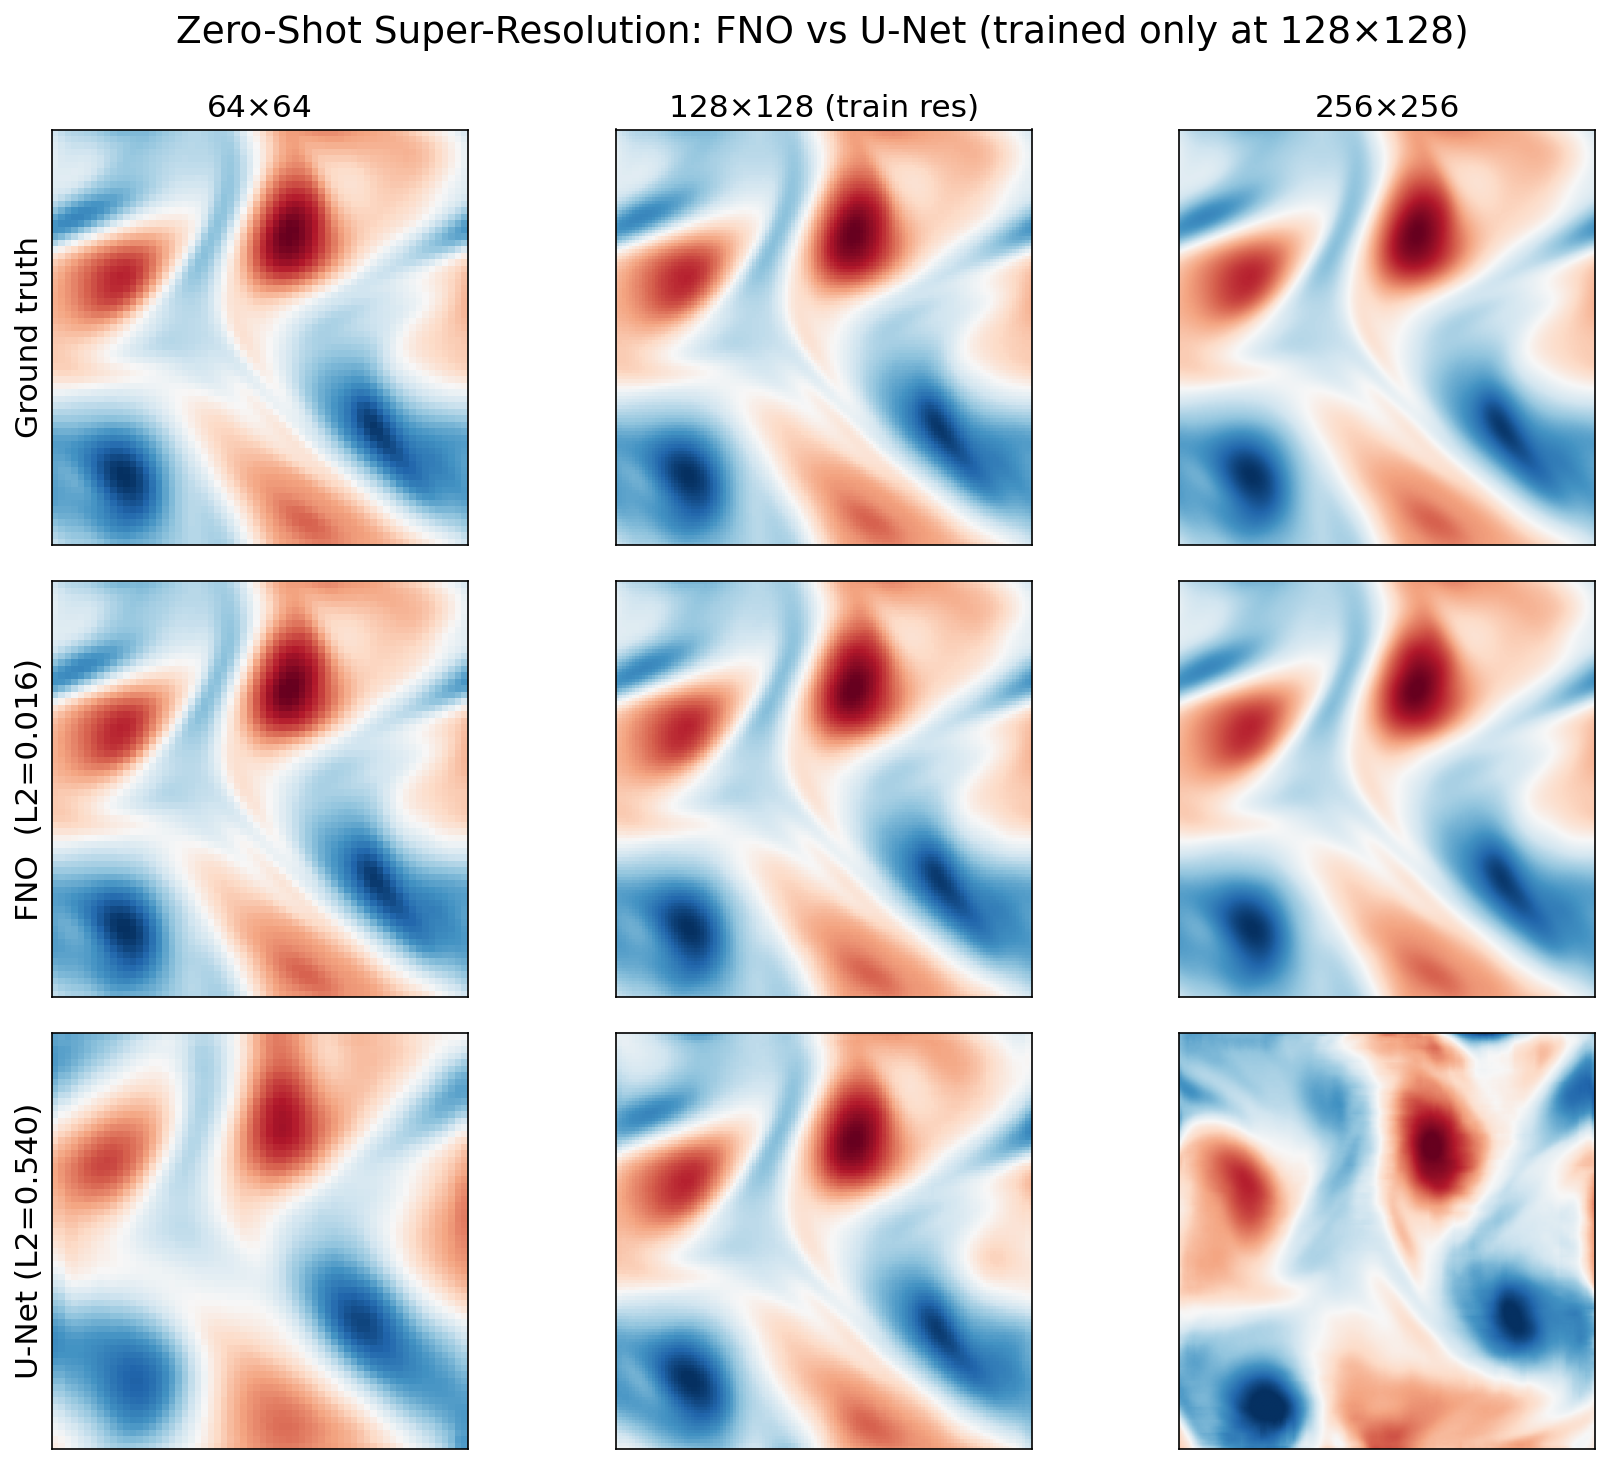
\includegraphics[width=\linewidth]{super_res.png}
  \caption{\textbf{Visual super-resolution comparison on one test sample.}
           \textbf{Columns:} $64\times64$, $128\times128$ (training res),
           $256\times256$.
           \textbf{Rows:} ground truth / FNO / U-Net.
           FNO looks sharp at every resolution.
           U-Net at $64\times64$ is blurry; at $256\times256$ it develops
           visible artefacts.}
  \label{fig:super_res}
\end{figure}

% ─── SECTION 6 ───────────────────────────────────────────────────────────────
\section{Discussion --- Why Did This Happen?}

\subsection{Why Did FNO Beat U-Net So Convincingly?}

The short answer: FNO's architecture \emph{matches the structure of the problem}.

Fluid dynamics is global.
A vortex forming on the left side of the domain immediately affects the pressure
everywhere, including the right side.
FNO's Fourier layers see the entire domain at once (via the FFT), so they can
naturally model these global interactions.

U-Net's $3 \times 3$ convolutions only look at a tiny neighbourhood at a time.
To propagate information from one side of a $128 \times 128$ field to the other,
you need many successive layers.
Even with 4 encoder levels, there is a limit to how much global context U-Net
can capture.

\begin{analogybox}
\textbf{Analogy.}
Imagine predicting traffic jams.
FNO is like having a helicopter view of the entire city at once.
U-Net is like standing on the ground looking through a small window ---
you can see what is nearby, but you miss the big picture.
Fluid dynamics needs the helicopter view.
\end{analogybox}

\subsection{Why Is FNO Resolution-Independent?}

FNO works in frequency space.
The Fourier Transform decomposes a signal into sine waves of different
frequencies.
Those frequencies have a fixed physical meaning (e.g., ``a swirl that repeats
4 times across the domain'') regardless of how finely the domain is sampled.

When you train FNO, it learns weights for ``how much to amplify each frequency
pattern.''
Those weights are valid at any resolution because the physical meaning of
the frequencies does not change.

U-Net's $3\times 3$ kernel, however, covers a \emph{physical} neighbourhood of
3 pixels $\times$ (grid spacing).
At $128 \times 128$ the grid spacing is $1/128$; at $256 \times 256$ it is
$1/256$.
The same kernel now covers half the physical area --- every learned filter has a
different physical meaning at the new resolution, which is why U-Net breaks.

\subsection{Parameter Efficiency}

FNO uses 6.6$\times$ fewer parameters but wins.
This is counterintuitive --- more parameters usually means more capacity.
But raw capacity is only useful if it is focused on the right things.

FNO's parameters are spent on learning the most important frequency components
of the fluid.
U-Net's 31 million parameters are spread across all the local pixel-to-pixel
relationships, most of which are redundant or irrelevant for the physics.

\subsection{What Are the Limitations?}

\begin{itemize}
  \item \textbf{Fixed viscosity.}
        Both models were trained at one viscosity value ($\nu = 10^{-4}$).
        We do not know if they generalise to thicker or thinner fluids.
  \item \textbf{Single-step only.}
        Small errors would accumulate over many timesteps --- we did not test this.
  \item \textbf{The super-resolution ``ground truth'' is approximate.}
        At $256 \times 256$, we created ground truth by bilinearly upsampling
        the $128 \times 128$ data. This is a reasonable proxy but not perfect.
\end{itemize}

% ─── SECTION 7 ───────────────────────────────────────────────────────────────
\section{Conclusion --- What Does It All Mean?}

We showed that:
\begin{enumerate}
  \item A neural network \emph{can} learn to predict fluid dynamics accurately
        from data alone, without solving the equations numerically.
  \item Designing the architecture to match the problem (Fourier layers for a
        Fourier-natured PDE) pays off enormously.
  \item FNO is more accurate, faster, smaller, and more flexible than U-Net.
  \item The resolution-independence of FNO is not a lucky side effect --- it
        is a direct consequence of how the architecture is built.
\end{enumerate}

The broader lesson is about \textbf{inductive bias}: if you bake the right
assumptions about your problem into your model's architecture, you can do more
with less data and fewer parameters.
This is especially powerful for physics problems where the underlying rules are
known and can be used to guide design.

% ─── GLOSSARY ─────────────────────────────────────────────────────────────────
\section*{Glossary of Terms}

\begin{description}
  \item[Vorticity] A measure of local rotation in a fluid.
        Positive = clockwise spin; negative = counter-clockwise spin.
  \item[Navier--Stokes equations] The PDEs that govern all viscous fluid flow.
        Derived in the 19th century; still unsolved analytically in the general
        turbulent case.
  \item[PDE (Partial Differential Equation)] An equation involving a function
        of multiple variables \emph{and} its derivatives.
        Describes how something changes across both space and time simultaneously.
  \item[Viscosity ($\nu$)] How ``thick'' a fluid is. Honey has high viscosity;
        water has low viscosity; air has very low viscosity.
  \item[Reynolds number (Re)] A dimensionless ratio of inertia to viscosity.
        High Re = turbulent. Our dataset: Re = 10{,}000 (very turbulent).
  \item[Neural operator] A neural network that maps functions to functions,
        not fixed-length vectors. Resolution-independent by design.
  \item[FNO] Fourier Neural Operator. Applies learned filters in frequency
        space (via FFT), enabling resolution-agnostic inference.
  \item[U-Net] A CNN encoder--decoder architecture with skip connections.
        Originally designed for medical image segmentation.
  \item[FFT (Fast Fourier Transform)] An efficient algorithm to convert a
        signal from the spatial domain to the frequency domain.
        Decomposes an image into sine waves of different frequencies.
  \item[Relative $L^2$ error] $\|\text{prediction} - \text{truth}\|_2 /
        \|\text{truth}\|_2$. Score of 1.0 = random guess; 0.0 = perfect.
  \item[Zero-shot super-resolution] Evaluating a model at a resolution it has
        never seen during training, without any fine-tuning.
  \item[Parameters / weights] The numbers inside a neural network adjusted
        during training. More parameters = more capacity (not always better).
  \item[Epoch] One complete pass through the entire training dataset.
  \item[Learning rate] How large a step the optimiser takes when updating
        parameters after each batch of training examples.
  \item[Cosine annealing] A learning rate schedule that starts high and
        gradually decays in a smooth cosine curve to near zero.
  \item[Inductive bias] Assumptions baked into a model's architecture about
        the structure of the problem. Good inductive bias = better performance
        with less data.
\end{description}

\end{document}
